\title{Lecture 3: Linear and Quadratic Equations and Inequalities}
\frame{\titlepage}

%%%%%%%%%%%%%
\section[Linear]{Linear Equation}
\frame{\sectionpage}
%%%%%%%%%%%%%

\begin{frame}
\begin{defn}{}{}
A \textbf{linear function} is of the form
\[ f(x) = ax + b \]
\end{defn}

\begin{exampleblock}{Examples of linear functions}
\begin{itemize}
\item $f(x) = x-2$
\item $f(x) = 3x + 1$
\item $\displaystyle f(x) = \frac{2}{3} x - \frac{4}{5}$
\item $f(x) = 1$ (in this case, $a=0$)
\end{itemize}
\end{exampleblock}
\end{frame}

\begin{frame}
\frametitle{How to solve a linear equation?}
Let $f(x) = ax + b$. The simplest form of linear equation is
\[ f(x) = c.\]
The goal is to find a real number $m$ such that $f(m) = c$. To achieve that, we want to rewrite the equation and derive
\[ x = \cdots\]
This can be achieved by using algebraic manipulation
\begin{eqnarray*}
ax + b &=& c \\
ax &=& c - \red{b}\\
x &=& \red{\frac{1}{a}}(c-b)
\end{eqnarray*}
\end{frame}

\begin{frame}[t]
\begin{ex}
Solve the following linear equations.
\begin{tasks}(2)
\task $2x+4=6$
\task $-3x-5=4$
\end{tasks}
\end{ex}
\begin{sol}

\begin{eqnarray*}
a) \quad 2x + 4 &=& 6 \\
2x &=& 6-4 = 2 \\
x &=& \frac{1}{2}\cdot  2 = 1 \\
b) \quad -3x -5 &=& 4 \\
-3x &=& 4+5 = 9 \\
x &=& \frac{1}{-3} \cdot 9 = -3
\end{eqnarray*}
\end{sol}
\end{frame}

\begin{frame}
Another form of linear equation is
\[ f(x) = g(x).\]
Here, we want to find a real number $m$ such that $f(m) = g(m)$. We can still use basic algebraic manipulations.
\begin{eqnarray*}
ax + b &=& cx + d \\ 
ax - \red{cx} &=& d - \red{b} \\
(a-c)x &=& d-b \\
x &=& \frac{d-b}{a-c}
\end{eqnarray*}
Note that we require $a-c\neq0$ or $a \neq c$. 
\end{frame}

\begin{frame}[t]
\begin{ex}
Solve the following linear equations.
\begin{tasks}(2)
\task $2x+4 =x-6$
\task $3x+5=x+7$
\end{tasks}
\end{ex}
\begin{sol}
\begin{eqnarray*}
a) \quad 2x + 4 &=& x - 6 \\
2x -x &=& -6-4 \\
x &=& -10 \\
b) \quad 3x+5 &=& x+7 \\
3x -x&=& 7-5 \\
2x &=& 2 \\
x &=& \frac{1}{2} \cdot 2 = 1
\end{eqnarray*}
\end{sol}
\end{frame}

\begin{frame}
\begin{exercisebox}{}{}
Solve the following linear equations
\begin{enumerate}
\item $x + 3 = 1$
\item $4x - 3 = 9$
\item $-2x - 5 = -8$
\end{enumerate}
Solve the following linear equations
\begin{enumerate}
\item $x + 3 = 2x-1$
\item $4x - 3 = -2x + 9$
\item $-2x - 5 = 3x - 8$
\end{enumerate}
\end{exercisebox}
\end{frame}

%%%%%%%%%%%%%
\section[System]{System of Equations}
\frame{\sectionpage}
%%%%%%%%%%%%%

\begin{frame}
\frametitle{System of Equations}
Let $a,b,c$ be real numbers and $x,y$ be variables. Consider a linear equation in two variables
\[ax + by = c.\] 
Since both $x$ and $y$ are unknown, there could be several solutions. For example, consider
\[ x+y=5.\]
We can see that $x=1$ and $y=4$ satisfies the equation, as well as $x=2$ and $y=3$, $x=10$ and $y=-5$, and so on and so forth.
\end{frame}

\begin{frame}
Suppose that we have two linear equations in two variables
\begin{eqnarray*}
a_1x+b_1y &=& c_1 \\
a_2x+b_2y &=& c_2.\\
\end{eqnarray*}
We can now attempt to solve it. We call this \textbf{a system of equations}. Depending on the values $a_1,b_1,c_1,a_2,b_2$ and $c_2$, there are three scenarios
\begin{remark}{Scenarios for a system of equations}
\begin{itemize}
\item There is no solution.
\item There is exactly one solution.
\item There are infinitely many solutions.
\end{itemize}
\end{remark}
\end{frame}


\begin{frame}[t]
We solve a system of equations by \textbf{eliminating} a variable. Suppose that we have
\begin{ex}
\begin{eqnarray}
x+y &=& 4\\
x-y &=& 2
\end{eqnarray}
\end{ex}
\begin{sol}
Then, we can eliminate $y$ by adding equation (2) to equation (1) to get
\begin{eqnarray*}
(x+y) + (x-y) &=& 4 + 2\\
2x &=& 6 \\
x &=& 3
\end{eqnarray*}
Since we have solved for $x$, we can use $x=3$ to solve for $y$ by using equation (1)
\[x +y=4 \rightarrow \quad 3+y = 4  \rightarrow \quad y = 1\]
\end{sol}
\end{frame}


\begin{frame}[t]
Usually, we need to multiply either equation by a real number so that the coefficients match. For example, 
\begin{ex}
\begin{eqnarray}
x+2y &=& 2\\
2x-y &=& 4
\end{eqnarray}
\end{ex}
\begin{sol}
Let's say we need to eliminate $y$. Then, we need to multiply equation (4) by $2$ to get
\begin{equation}
4x - 2y = 8
\end{equation} 
Now, we can add equation (3) to equation (5) to get
\begin{eqnarray*}
(x+2y) + (4x-2y) &=& 2 + 8\\
5x &=& 10 \rightarrow x = 2
\end{eqnarray*}
We can plug in $x=2$ into equation (3) to get $2 + 2y = 2$ and thus $y = 0$.
\end{sol}
\end{frame}


\begin{frame}[t]
\begin{ex}
\begin{eqnarray}
2x+3y &=& 4\\
5x+4y &=& 3
\end{eqnarray}
\end{ex}
\begin{sol}
Let's say we need to eliminate $y$. Then, we need a real number $m$ such that
\[ 3y + 4my = 0\]
Solving for $m$ yields 
\[ m = -\frac{3}{4}\]
Thus, we need to multiply equation (7) by $-\frac{3}{4}$ to get
\begin{equation}
-\frac{15}{4}x - 3y = -\frac{9}{4}
\end{equation} 
\end{sol}
\end{frame}

\begin{frame}
\begin{sol}
Adding equation (6) to equation (8) yields
\begin{eqnarray*}
(2x+3y) + \left(-\frac{15}{4}x - 3y \right) &=& 4 + \left(-\frac{9}{4}\right)\\
\frac{8x}{4} - \frac{15}{4} &=& \frac{16}{4} - \frac{9}{4} \\
8x-15x &=& 7 \\
x &=& \frac{7}{-7} = -1
\end{eqnarray*}
We can plug in $x= 1$ into equation (6) to get 
\[ 2(-1) + 3y = 4 \rightarrow \quad  3y = 4 - (2)(-1)  \rightarrow \quad y = 3\]
\end{sol}
\end{frame}

\begin{frame}
\begin{exercisebox}{}{}
Solve the following systems of equations.
\begin{enumerate}
\item
\begin{eqnarray*}
x + y &=& 6\\
2x - y &=& 3
\end{eqnarray*}
\item
\begin{eqnarray*}
2x + 3y &=& 7 \\
4x - 3y &=& 5
\end{eqnarray*}
\item
\begin{eqnarray*}
3x + 4y &=& 6 \\
2x - 5y &=& -1
\end{eqnarray*}
\end{enumerate}
\end{exercisebox}
\end{frame}

%%%%%%%%%%%%%
\section[Quadratic]{Quadratic Equation}
\frame{\sectionpage}
%%%%%%%%%%%%%

\begin{frame}
\frametitle{How to solve a quadratic equation?}
\begin{defn}{}{}
A \textbf{quadratic function} is of the form
\[ f(x) = ax^2+bx +c\]
\end{defn}

There are three ways to find the roots of a quadratic equation.

\begin{enumerate}
\item Using the formula
\item Factoring
\item Completing a square
\end{enumerate}
\end{frame}

\begin{frame}
\frametitle{1 - Using the Formula}
\begin{thm}{}{}
A quadratic function $f(x) = ax^2 + bx + c$ has two roots
\[ x =  \frac{-b \pm \sqrt{b^2 - 4ac}}{2a}.\]

In particular, the roots are
\begin{eqnarray*}
m_1 &=& \frac{-b + \sqrt{b^2 - 4ac}}{2a} \text{ and } \\
m_2 &=& \frac{-b - \sqrt{b^2 - 4ac}}{2a} 
\end{eqnarray*}
\end{thm}
\end{frame}


\begin{frame}[t]
\begin{ex}
Find the roots of $x^2 - 2x - 3=0$.
\end{ex}
\begin{sol}
By comparing to the form $ax^2 + bx + c$, we get $a = 1, b = -2,  c = -3$. Thus, we can plug these values into the formula
\begin{eqnarray*}
x  = \frac{-b \pm \sqrt{b^2 - 4ac}}{2a} &=& \frac{-(-2) \pm \sqrt{(-2)^2 - 4(1)(-3)}}{2(1)} \\
&=& \frac{2 \pm \sqrt{16}}{2} = \frac{2 \pm 4}{2}
\end{eqnarray*}
So the roots are
\[ m_1 = \frac{2+4}{2} = 3, \qquad m_2 = \frac{2-4}{2} = -1\]
\end{sol}
\end{frame}


\begin{frame}[t]
\begin{ex}
Find the roots of $2x^2 - 3x -2=0$.
\end{ex}
\begin{sol}
By comparing to the form $ax^2 + bx + c$, we get $a = 2, b = -3, c = -2$. Thus, we can plug these values into the formula
\begin{eqnarray*}
x  = \frac{-b \pm \sqrt{b^2 - 4ac}}{2a} &=& \frac{-(-3) \pm \sqrt{(-3)^2 - 4(2)(2)}}{2(2)} \\
&=& \frac{3 \pm \sqrt{25}}{2} = \frac{3 \pm 5}{4}
\end{eqnarray*}
So the roots are
\[ m_1 = \frac{3+5}{4} = 2, \qquad m_2 = \frac{3-5}{4} = -\frac{1}{2}\]
\end{sol}
\end{frame}

\begin{frame}
\begin{exercisebox}{}{}
Find the roots following quadratic functions using the formula
\[ x =  \frac{-b \pm \sqrt{b^2 - 4ac}}{2a}.\]
\begin{enumerate}
\item $f(x) = x^2 +5x+6$
\item $f(x) = x^2 - x - 12$
\item $f(x) = 3x^2 +5x - 2$
\end{enumerate}
\end{exercisebox}
\end{frame}


\begin{frame}
\frametitle{2 - Factoring}
Suppose we have $f(x) = x^2 +bx+c$ where the coefficient of $x^2$ is 1. Also, suppose that $f(x)$ can be written as $f(x) = (x-m_1)(x-m_2)$. Then, it is immediate that $x=m_1$ and $x=m_2$ are the roots of $f(x)$ since
\[ f(m_1) = (m_1-m_1)(m_1-m_2) = 0\]
\[ f(m_2) = (m_2-m_1)(m_2-m_2) = 0\]
We can now work backward. By expanding the product, we get
\[ f(x) = (x-m_1)(x-m_2) = x^2 -m_1x - m_2x + m_1m_2 = x^2 - (m_1+m_2)x + m_1m_2\]
By comparing the coefficients to the original $x^2 + bx + c$, we know that
\begin{eqnarray*}
m_1+m_2 &=& -b\\
m_1m_2 &=& c
\end{eqnarray*}
\end{frame}

\begin{frame}
Hence, if we can find $m_1$ and $m_2$ that satisfy 
\begin{block}{}
\begin{eqnarray*}
m_1+m_2 &=& -b\\
m_1m_2 &=& c
\end{eqnarray*}
\end{block}
Then $m_1$ and $m_2$ are the roots of $f(x)$. Nevertheless, this method works if $b,c$ are small and if $m_1,m_2$ are integers.
\bigskip

Note: If the function is of the form $f(x) = ax^2 + bx + c$ when $a \neq 1$, then we can use a slightly modified method, which we won't cover here.
\end{frame}



\begin{frame}[t]
\begin{ex}
Find the roots of $x^2+4x+3=0$.
\end{ex}
\begin{sol}
Let $f(x) = x^2 +4x+3$. We want to find $m_1,m_2$ such that
\begin{eqnarray*}
m_1 + m_2 &=& -b = -4 \\
m_1m_2 &=& c = 3.
\end{eqnarray*}
Since 3 is a prime number, our guesses would be 
\begin{itemize}
\item $m_1 = 1$ and $m_2 = 3$. In this case, $m_1 + m_2 = 1+3=4 \neq -4$ so this guess fails.
\item or $m_1 = -1$ and $m_2 = -3$. In this case, $m_1 + m+2 = -1+-3 = -4$
\end{itemize}
Thus, $m_1 = -1$ and $m_2 = -3$ are roots of $f(x) = x^2 + 4x + 3$.
\end{sol}
\end{frame}


\begin{frame}[t]
\begin{ex}
Find the roots of $ x^2 -7x+12=0$.
\end{ex}
\begin{sol}
Let $f(x) = x^2 -7x+12$. We want to find $m_1,m_2$ such that
\begin{eqnarray*}
m_1 + m_2 &=& -b = 7 \\
m_1m_2 &=& c = 12.
\end{eqnarray*}
Notice that $12 = 2 \times 2 \times 3$, so there are many ways to factor $12$ into a product of two integers. Let's create a table to consider all possibilities.
\begin{table}
\centering
\begin{tabular}{|C||C|C|C|C|C|C|}
\hline
m_1 & -3 & -2 & -1 & 1 & 2 & 3 \\
\hline
m_2 & -4 & -6 & -12 & 12 & 6 & 4 \\
\hline \hline
m_1 +m_2 & -7 & -8 & -13 & 13 & 8 & 7 \\
\hline
\end{tabular}
\end{table}
Thus, $m_1 = 3$ and $m_2 = 4$ are roots of $f(x) = x^2 -7x + 12$.
\end{sol}
\end{frame}

\begin{frame}
\begin{exercisebox}{}{}
Find the roots of the following quadratic functions by factoring
\[(x-m_1)(x-m_2) = x^2 - (m_1+m_2)x + m_1m_2.\]
\begin{enumerate}
\item $f(x) = x^2 +3x+2$
\item $f(x) = x^2 + 7x - 18$
\item $f(x) = 3x^2 +5x - 2$
\end{enumerate}
\end{exercisebox}
\end{frame}

\begin{frame}
\frametitle{3 - Completing a square}
This method is the most intuitive as it works similarly to solving a linear equation. Moreover, this method generates the formula shown in the first method.

Let $f(x) = ax^2 + bx + c$ be a quadratic equation. By using the identity that $(x-m)^2 = x^2 - 2mx + m^2$, we have
\begin{eqnarray*}
ax^2 + bx + c &=& a\left(x^2 + \frac{b}{a}x + \frac{c}{a} \right) \\
&=& a \left(x^2 + 2\frac{b}{a}x + \left(\frac{b}{2a}\right)^2 - \left(\frac{b}{2a}\right)^2 + \frac{c}{a} \right) \\
&=& a\left( \left(x - \frac{b}{2a}\right)^2- \left( \frac{b^2}{4a^2} - \frac{c}{a}\right)  \right)
\end{eqnarray*}
\end{frame}

\begin{frame}
We can rewrite $ \frac{b^2}{4a^2} - \frac{c}{a}$ as a square.
\begin{eqnarray*}
a\left( \left(x - \frac{b}{2a}\right)^2- \left( \frac{b^2}{4a^2} - \frac{c}{a}\right)  \right) &=&  a\left( \left(x - \frac{b}{2a}\right)^2- \left( \frac{b^2-4ac}{4a^2}\right)  \right) \\
&=& a\left( \left(x - \frac{b}{2a}\right)^2- \left( \frac{\sqrt{b^2-ac}}{2a}\right)^2  \right)
\end{eqnarray*}
To simplify, let $\frac{\sqrt{b^2-4ac}}{2a} = D$. Then, we use the identity $x^2 - m^2 = (x-m)(x+m)$ to rewrite it as
\begin{eqnarray*}
a\left( \left(x - \frac{b}{2a}\right)^2- \left( \frac{\sqrt{b^2-4ac}}{2a}\right)^2  \right) & = & a\left( \left(x - \frac{b}{2a}\right)^2- D^2  \right) \\
&=& a\left( x - \frac{b}{2a} - D\right) \left(x - \frac{b}{2a} + D \right)
\end{eqnarray*}
\end{frame}

\begin{frame}
Therefore, we now find two roots of the function $f(x)$, namely
\begin{block}{}
\[ x = \frac{b}{2a} - D, \quad  \frac{b}{2a} + D\]
\end{block}

In practice, all these variables $a,b,c$ will be combined into a single real number, so it won't look as messy as this.
\end{frame}


\begin{frame}[t]
\begin{ex}
Find the roots of $  x^2 +6x+8=0$.
\end{ex}
\begin{sol}
Let $f(x) = x^2 +6x+8$. We can complete a square and solve for the roots as follows.
\begin{eqnarray*}
x^2 + 6x + 8 &=& x^2 + 2(3x) + 3^2 - 3^2 + 8 \\
&=& (x-3)^2 - 1 \\
&=& ((x-3)-1)((x-3)+1) \\
&=& (x-4)(x-2)
\end{eqnarray*}
Hence, the roots are $x = -4$ and $x=2$.
\end{sol}
\end{frame}


\begin{frame}[t]
\begin{ex}
Find the roots of $   x^2 -8x-20=0$.
\end{ex}
\begin{sol}
Let $f(x) = x^2 -8x-20$. We can complete a square and solve for the roots as follows.
\begin{eqnarray*}
x^2 - 8x -20 &=& x^2 + 2(-4x) + (-4)^2 - (-4)^2 - 20 \\
&=& (x-(-4))^2 - 36 \\
&=& (x+4)^2 - 6^2 \\
&=& ((x+4)-6)((x+4)+6) \\
&=& (x-2)(x+10)
\end{eqnarray*}
Hence, the roots are $x = 2$ and $x=-10$.
\end{sol}
\end{frame}

\begin{frame}
\begin{exercisebox}{}{}
Find the roots of the following quadratic functions by completing a square.
\[ (x+a)^2 = x^2 +2ax + a^2\]
%\[ x^2 - b^2 = (x-b)(x+b)\]
\begin{enumerate}
\item $f(x) = x^2 -4x+4$
\item $f(x) = x^2 +6x -16$
\item $f(x) = x^2 - x - 2$
\end{enumerate}
\end{exercisebox}
\end{frame}


%%%%%%%%%%%%%
\section{Inequality}
\frame{\sectionpage}
%%%%%%%%%%%%%


\begin{frame}
\frametitle{Motivation}
\addfig{0.8}{ineq_hitbox}{Hitboxes in Mario}{}
\end{frame}


\begin{frame}
\frametitle{Keywords}
Comparison (greater, smaller), superlative (greatest, smallest) \pause
\bigskip

\[ <, \quad >, \quad \leq, \quad \geq\]

\begin{remark}{}
\begin{itemize}
\item ``$a$ is greater than $b$'' means $a > b$.
\item ``$a$ is greater than or equal to $b$'' means $a \geq b$.
\item ``$a$ is at least $b$'' means $a \geq b$.
\end{itemize}
\end{remark}
\end{frame}

\begin{frame}
\frametitle{Inequality and Set}
We can use interval notation to represent the set of solutions of an inequality.
\begin{defn}{}{}
Let $a$ and $b$ be real numbers.
\begin{eqnarray*}
x < a \pause &\longrightarrow& x \in (-\infty, a) \\ \pause
x \leq a &\longrightarrow& x \in (-\infty, a] \\ \pause
x > a \pause &\longrightarrow& x \in (a, \infty) \\ \pause
x \geq a &\longrightarrow& x \in [a, \infty) \\ \pause
\bigskip \\
a < x < b \pause &\longrightarrow& x \in (a,b) \\ \pause
x < a \text{ or } x > b \pause &\longrightarrow& x \in (-\infty, a) \cup (b, \infty)
\end{eqnarray*}
\end{defn}
\end{frame}

\begin{frame}
\begin{figure}[h!]
\centering
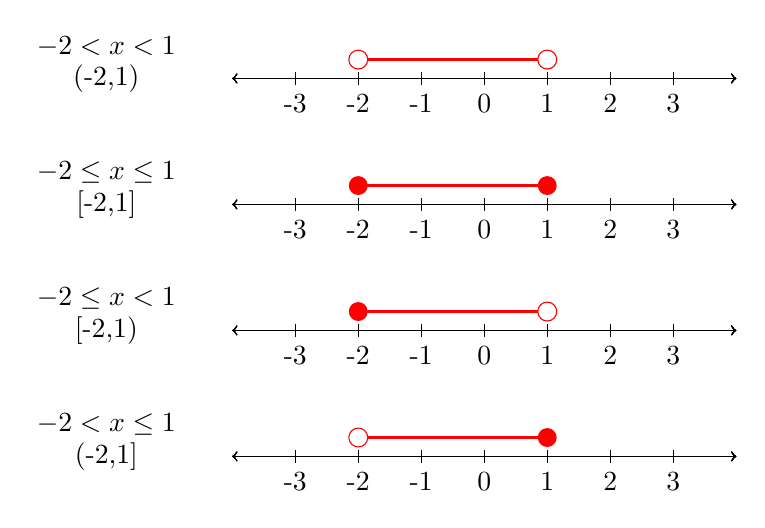
\begin{tikzpicture}[scale=0.8]
\foreach \y in {0,2,4,6}
{
	\draw[red, thick] (-2,\y+0.3) -- (1,\y+0.3);
	\foreach \x in {-3, -2, -1,..., 3} {
		\draw[<->] (-4,\y) -- (4,\y);
		\draw (\x,\y+0.1) -- (\x,\y-0.1) node[anchor = north] {\x};
	}
}
\begin{scope}[xshift = -60mm]
\node at (0,6) {(-2,1)};
\node at (0,6.5) {$-2<x<1$};
\node at (0,4) {[-2,1]};
\node at (0,4.5) {$-2 \leq x \leq 1$};
\node at (0,2) {[-2,1)};
\node at (0,2.5) {$-2 \leq x<1$};
\node at (0,0) {(-2,1]};
\node at (0,0.5) {$-2 < x\leq 1$};
\end{scope}
\foreach \x / \y in {-2/6, 1/6, 1/2, -2/0}
	\filldraw[draw = red, fill = white] (\x,\y+0.3) circle (1.5mm);
\foreach \x / \y in {-2/4, 1/4, -2/2, 1/0}
	\fill[red] (\x,\y+0.3) circle (1.5mm);
\end{tikzpicture}
\caption{Types of intervals}
\end{figure}
\end{frame}

\begin{frame}
\begin{figure}[h!]
\centering
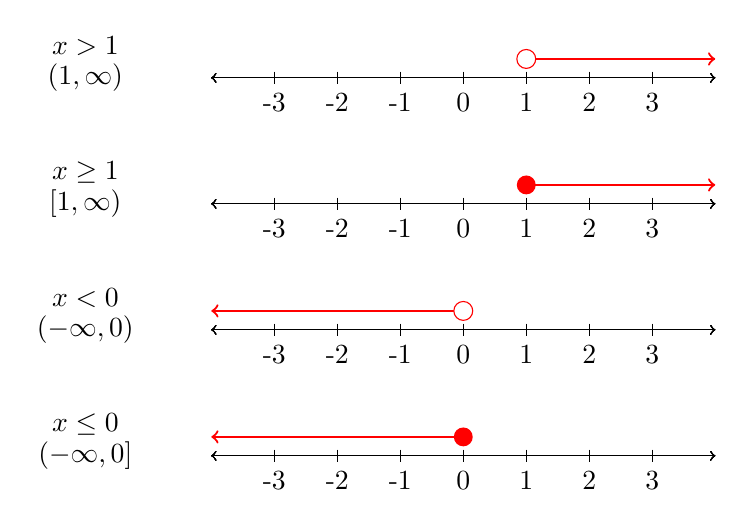
\begin{tikzpicture}[scale=0.8]
\foreach \y in {0,2,4,6}
{
	\foreach \x in {-3, -2, -1,..., 3} {
		\draw[<->] (-4,\y) -- (4,\y);
		\draw (\x,\y+0.1) -- (\x,\y-0.1) node[anchor = north] {\x};
	}
}
\draw[->, red, thick] (1,6.3) -- (4,6.3);
\draw[->, red, thick] (1,4.3) -- (4,4.3);
\draw[->, red, thick] (0,2.3) -- (-4,2.3);
\draw[->, red, thick] (0,0.3) -- (-4,0.3);
\begin{scope}[xshift = -60mm]
\node at (0,6) {$(1, \infty)$};
\node at (0,6.5) {$x > 1$};
\node at (0,4) {$[1, \infty)$};
\node at (0,4.5) {$x \geq 1$};
\node at (0,2) {$(-\infty, 0)$};
\node at (0,2.5) {$x < 0$};
\node at (0,0) {$(-\infty,0]$};
\node at (0,0.5) {$x \leq 0$};
\end{scope}
\foreach \x / \y in {1/6, 0/2}
	\filldraw[draw = red, fill = white] (\x,\y+0.3) circle (1.5mm);
\foreach \x / \y in {1/4, 0/0}
	\fill[red] (\x,\y+0.3) circle (1.5mm);
\end{tikzpicture}
\caption{Types of intervals}
\end{figure}
\end{frame}


\begin{frame}
\frametitle{Compound Inequality}
One statement may include more than one inequality. For instance,
\[0 < x \leq 2\]
means
\[0 < x \quad \text{ and } x \leq 2.\]
Even though usually you can solve both equations altogether, it is recommended to solve each of them separately and find the common solution using set intersection.
\end{frame}

\begin{frame}
\begin{exercisebox}{}{}
Express the solutions to the following inequalities using interval notation.
\begin{enumerate}
\item $x \leq 3$
\item $x > 2$
\end{enumerate}
Write down an inequality whose solutions are the following intervals.
\begin{enumerate}
\item $(2, \infty)$
\item $(-\infty, -3]$
\item $[0.5, 1.5)$
\item $(-\infty, 1) \cup (2, \infty)$
\end{enumerate}

\end{exercisebox}
\end{frame}


%%%%%%%%%%%%%
\section{Linear Inequality}
\frame{\sectionpage}
%%%%%%%%%%%%%

\begin{frame}
\frametitle{Addition Property}
\begin{thm}{}{}
For any real numbers $a,b$, if
\[a<b,\]
then for any real number $c$ we have
\[a + \red{c} < b + \red{c}.\]
Moreover, these properties also apply to $a \leq b, a > b$ and $a \geq b$.
\end{thm}
\end{frame}

\begin{frame}
\begin{figure}[h!]
\centering
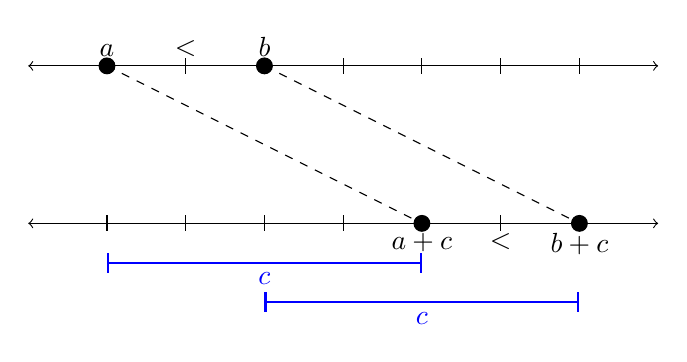
\begin{tikzpicture}
\foreach \y in {0,2}
{
	\draw[<->] (-4,\y) -- (4,\y);
	\foreach \x in {-3,-2,...,3} 
	{
		\draw (\x, \y+0.1) -- (\x, \y-0.1); %node[anchor = north] {\x};
	}
}
\filldraw (-3,2) circle (1mm) node[above] {$a$};
\node[above] at (-2,2) {$<$};
\filldraw (-1,2) circle (1mm) node[above] {$b$};
\filldraw (1,0) circle (1mm) node[below] {$a+c$};
\node[below] at (2,0) {$<$};
\filldraw (3,0) circle (1mm) node[below] {$b+c$};
\draw[dashed] (-3,2) -- (1,0);
\draw[dashed] (-1,2) -- (3,0);
\draw[blue, |-|, thick] (-3,-0.5) -- (1,-0.5) node[below, pos=0.5] {$c$};
\draw[blue, |-|, thick] (-1,-1) -- (3,-1) node[below, pos=0.5] {$c$};
\end{tikzpicture}
\caption{The addition property}
\end{figure}
\end{frame}


\begin{frame}[t]
\begin{ex}
Find the solutions of the following inequalities.
\begin{tasks}(2)
\task $x-5 \leq 10$
\task $x+1 > -4$
\end{tasks}
\end{ex}
\begin{sol}
\begin{tasks}(2)
\task 
\begin{eq*}
x - 5 &\leq& 10 \\
x-5 + 5 &\leq& 10+5\\ 
x &\leq& 15 \\
x &\in& (-\infty, 15]
\end{eq*}
\task
\begin{eq*}
x +1 &>& -4 \\
x+1-1 &>& -4-1\\ 
x &>& -5 \\
x &\in& (-5,\infty)
\end{eq*}
\end{tasks}
\end{sol}
\end{frame}

\begin{frame}
\frametitle{Multiplication Property}
\begin{thm}{}{}
\begin{itemize}
\item For any real number $a$ and positive real number $b$,
\[\text{ if } \quad x<a, \text{ then} \quad bx < ba.\]
\item For any real number $a$ and \red{negative} real number $b$,
\[\text{ if } \quad x<a, \text{ then} \quad bx\, \red{ > }\,  ba.\]
\end{itemize}
Moreover, these properties also apply to $a \leq b, a > b$ and $a \geq b$.
\end{thm}
\end{frame}

\begin{frame}
\begin{figure}[h!]
\centering
\begin{tikzpicture}
\foreach \y in {0,2}
{
	\draw[<->] (-1,\y) -- (9,\y);
	\foreach \x in {0,1,...,8} 
	{
		\draw (\x, \y+0.1) -- (\x, \y-0.1); %node[anchor = north] {\x};
	}
}
\node[above] at (0,2) {$0$};
\node[above] at (1,2) {$1$};
\filldraw (2,2) circle (1mm) node[above] {$a$};
\node[above] at (3,2) {$<$};
\filldraw (4,2) circle (1mm) node[above] {$b$};
\node[above] at (0,0) {$0$};
\node[below] at (2,0) {$c$};
\filldraw (4,0) circle (1mm) node[below] {$ca$};
\node[below] at (6,0) {$<$};
\filldraw (8,0) circle (1mm) node[below] {$cb$};
\draw[dashed] (0,4) -- (0,0);
\draw[dashed] (0,4) -- (2,0);
\draw[dashed] (0,4) -- (4,0);
\draw[dashed] (0,4) -- (8,0);
\draw[blue, |-|, thick] (0,-0.5) -- (2,-0.5) node[below, pos=0.5] {$c$};
\end{tikzpicture}
\caption{The multiplication property when $c$ is positive}
\end{figure}
\begin{center}
If $a < b$ and $c$ is positve, then $ca < cb$.
\end{center}
\end{frame}


\begin{frame}
\begin{figure}[h!]
\centering
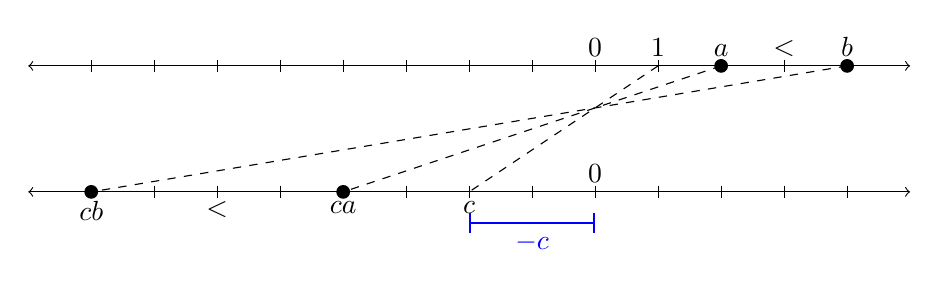
\begin{tikzpicture}[scale=0.8]
\foreach \y in {0,2}
{
	\draw[<->] (-9,\y) -- (5,\y);
	\foreach \x in {-8, -7,...,4} 
	{
		\draw (\x, \y+0.1) -- (\x, \y-0.1); %node[anchor = north] {\x};
	}
}
\node[above] at (0,2) {$0$};
\node[above] at (1,2) {$1$};
\filldraw (2,2) circle (1mm) node[above] {$a$};
\node[above] at (3,2) {$<$};
\filldraw (4,2) circle (1mm) node[above] {$b$};
\node[above] at (0,0) {$0$};
\node[below] at (-2,0) {$c$};
\filldraw (-4,0) circle (1mm) node[below] {$ca$};
\node[below] at (-6,0) {$<$};
\filldraw (-8,0) circle (1mm) node[below] {$cb$};
\draw[dashed] (1,2) -- (-2,0);
\draw[dashed] (2,2) -- (-4,0);
\draw[dashed] (4,2) -- (-8,0);
\draw[blue, |-|, thick] (0,-0.5) -- (-2,-0.5) node[below, pos=0.5] {$-c$};
\end{tikzpicture}
\caption{The multiplication property when $c$ is negative}
\end{figure}
\begin{center}
If $a < b$ and $c$ is negative, then $ca > cb$.
\end{center}
\end{frame}


\begin{frame}[t]
\begin{ex}
Find the solutions of the following inequalities.
\begin{tasks}(2)
\task $2x \leq 10$
\task $4x+1 > 5$
\end{tasks}
\end{ex}
\begin{sol}
\begin{tasks}(2)
\task 
\begin{eq*}
2x &\leq& 10 \\
\frac{1}{2} (2x) &\leq& \frac{1}{2}(10)\\ 
x &\leq& 5 \\
x &\in& (-\infty, 5]
\end{eq*}
\task
\begin{eq*}
4x +1 &>& 5 \\
4x+1-1 &>& 5-1\\ 
4x &>& 4 \\
\frac{1}{4} x &>& \frac{1}{4} (4) \\
x &>& 1 \\
x &\in& (1,\infty)
\end{eq*}
\end{tasks}
\end{sol}
\end{frame}



\begin{frame}[t]
\begin{ex}
Find the solutions of the following inequalities.
\begin{tasks}(2)
\task $-2x+2 \leq 10$
\task $-3x > 4$
\end{tasks}
\end{ex}
\begin{sol}
\begin{tasks}(2)
\task 
\begin{eq*}
-2x+2 &\leq& 10 \\
-2x &\leq& 8\\ 
x &\red{\geq}& -4 \\
x &\in& (-4, \infty)
\end{eq*}
\task
\begin{eq*}
-3x &>& 4 \\
x &\red{<}& -\frac{4}{3}\\ 
x &\in& \left(-\infty, \frac{4}{3}\right)
\end{eq*}
\end{tasks}
\end{sol}
\end{frame}

\begin{frame}
\begin{exercisebox}{}{}
Find the set of solutions for each of the following inequalities.
\begin{enumerate}
\item $x + 3 < 5$
\item $3x + 4 \geq -1$
\item $-x + 4 > 2$
\item $-4x - 6 \leq 10$
\end{enumerate}
\end{exercisebox}
\end{frame}



\begin{frame}[t]
\begin{ex}
Let Mario be at position $x$, and let Koopa occupy the closed interval $[1,4]$ at the same height as Mario. Suppose Mario's hitbox is a closed interval from one unit to the left and one unit to right of his position.
\begin{tasks}(1)
\task Draw Koopa's and Mario's hitboxes on the real line when Mario's position is at $x=6$.
\task Describe the inequalities where Mario's hitbox \textbf{does not} overlap with Koopa.
\task Find the solutions.
\end{tasks}
\end{ex}
\addfig{0.7}{ineq_abs_mario_ex.png}{}{}
\end{frame}

\begin{frame}
\begin{sol}
\begin{tasks}(1)
\task Here.
\begin{figure}[h!]
\centering
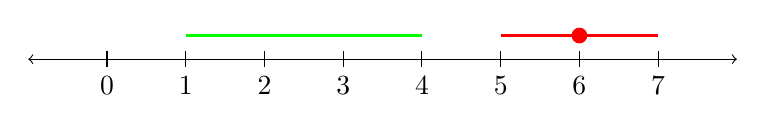
\begin{tikzpicture}
\foreach \x in {0,1,...,7} 
{
	\draw (\x, 0.1) -- (\x, -0.1) node[anchor = north] {\x};
}
\draw[<->] (-1,0) -- (8,0);
\draw[green, thick] (1,0.3) -- (4,0.3);
\draw[red, thick] (5,0.3) -- (7,0.3);
\fill[red] (6,0.3) circle (1mm);
\end{tikzpicture}
\caption{Positions of Koopa and Mario}
\end{figure}
\task There are two possible scenario.
\begin{itemize}
\item The edge on the left of Mario's hitbox is to the right of Koopa's interval. This means that we have
\[x-1 > 4,\]
\item On the other hand, it's also possible that the edge on the right of Mario's hitbox is to the left of Koopa's interval. This means we have
\[x+1 < 1.\]
\end{itemize}
\end{tasks}
\end{sol}
\end{frame}

\begin{frame}
\begin{sol}
\begin{tasks}(1)
\task Combining both inequalities, we obtain
\[x < 0 \quad \text{or} \quad x > 5.\]
In interval notation, we have $x \in (-\infty, 0) \cup (5, \infty)$.
\end{tasks}
\begin{figure}[h!]
\centering
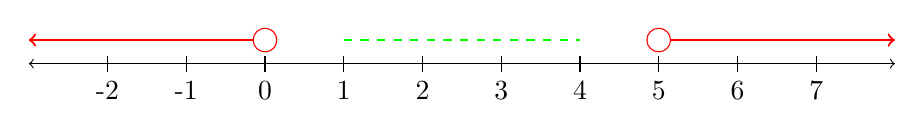
\begin{tikzpicture}
\foreach \x in {-2,-1,...,7} 
{
	\draw (\x, 0.1) -- (\x, -0.1) node[anchor = north] {\x};
}
\draw[<->] (-3,0) -- (8,0);
\draw[dashed, green, thick] (1,0.3) -- (4,0.3);
\draw[->, red, thick] (5,0.3) -- (8,0.3);
\draw[->, red, thick] (0,0.3) -- (-3,0.3);
\filldraw[fill = white, draw = red] (0,0.3) circle (1.5mm);
\filldraw[fill = white, draw = red] (5,0.3) circle (1.5mm);
\end{tikzpicture}
\caption{The intervals of positions where Mario is safe.}
\end{figure}
\end{sol}
\end{frame}



%%%%%%%%%%%%%
\section[Absolute Ineq]{Absolute Value Inequality}
\frame{\sectionpage}
%%%%%%%%%%%%%



\begin{frame}
\frametitle{Absolute Value Function}
\begin{defn}{}{}
Define the absolute value function 
\[|x| = \begin{cases} x \quad &\text{ if } x \geq 0 \\ -x \quad &\text{ if } x < 0 \end{cases}\]
\end{defn}
\begin{ex}
\[|3| = 3, \quad |-4| = 4, \quad |0| = 0\]
\end{ex}
\end{frame}

\begin{frame}
\frametitle{Alternate Definition: Distance Between Points}
Simple absolute value inequality can be solved directly from the definition.
\begin{defn}{}{}
Let $a$ be a real number. The function
\[f(x) = |x - a|\]
is equals to the distance between the points $x$ and $a$ on the real line.
\end{defn}
\end{frame}


\begin{frame}[t]
\begin{ex}
Solve the following absolute value inequality
\[|x-4| < 2.\]
\end{ex}
\begin{sol}
The inequality is the set of real numbers $x$ such that the distance between $x$ and 4 is less than 2. 
\begin{figure}[h!]
\centering
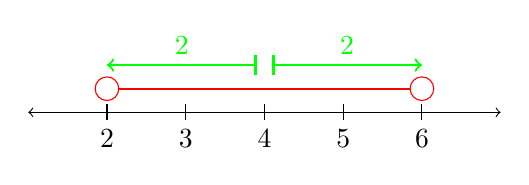
\begin{tikzpicture}
\foreach \x in {2,3,...,6} 
{
	\draw (\x, 0.1) -- (\x, -0.1) node[anchor = north] {\x};
}
\draw[<->] (1,0) -- (7,0);
\draw[<-|, green, thick] (2,0.6) -- (3.9,0.6) node[above, pos=0.5] {2};
\draw[|->, green, thick] (4.1,0.6) -- (6,0.6) node[above, pos=0.5] {2};
\draw[red, thick] (2,0.3) -- (6,0.3);
\filldraw[fill = white, draw = red] (2,0.3) circle (1.5mm);
\filldraw[fill = white, draw = red] (6,0.3) circle (1.5mm);
\end{tikzpicture}
\caption{The interval solution of $|x-4| < 2$}
\end{figure}

We can find the interval on the real line to be $(2,6)$, thus $x \in (2,6)$.
\end{sol}
\end{frame}


\begin{frame}[t]
\begin{ex}
Solve the following absolute value inequality
\[|x+3| \geq 3.\]
\end{ex}
\begin{sol}
First, rewrite the function as $|x+3| = |x - (-3)|$. 

Then, the inequality is the set of real numbers $x$ such that the distance between $x$ and $-3$ is greater than or equals to 3. 

\begin{figure}[h!]
\centering
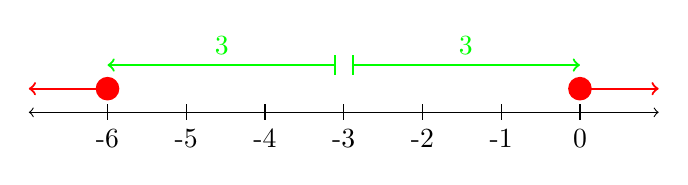
\begin{tikzpicture}
\foreach \x in {-6,-5,...,0} 
{
	\draw (\x, 0.1) -- (\x, -0.1) node[anchor = north] {\x};
}
\draw[<->] (-7,0) -- (1,0);
\draw[<-|, green, thick] (-6,0.6) -- (-3.1,0.6) node[above, pos=0.5] {3};
\draw[|->, green, thick] (-2.9,0.6) -- (0,0.6) node[above, pos=0.5] {3};
\draw[<-, red, thick] (-7,0.3) -- (-6,0.3);
\draw[->, red, thick] (0,0.3) -- (1,0.3);
\fill[red] (-6,0.3) circle (1.5mm);
\fill[red] (0,0.3) circle (1.5mm);
\end{tikzpicture}
\caption{The interval solution of $|x+3| \geq 3$}
\end{figure}

Thus, the solutions are $x \in (-\infty,6) \cup (0, \infty)$.
\end{sol}
\end{frame}

\begin{frame}
\frametitle{Absolute Value Inequality}
In general, you can solve an absolute value inequality first by getting rid of the absolute value as follows.
\begin{defn}{}{}
For functions $f(x)$ and $g(x)$, an absolute value inequality is an inequality of the form:
\begin{enumerate}
\item $| f(x) | < g(x)$. This is equivalent to 
\[-g(x) < f(x) < g(x), \text{ or } -g(x) < f(x) \text{ and } f(x) < g(x).\]
\item $|f(x)| > g(x)$. This is equivalent to 
\[f(x) < -g(x) \text{ or } f(x) > g(x).\]
\end{enumerate}
These statements also apply to $|f(x)| \leq k$ and $|f(x)| \geq k$.
\end{defn}
\end{frame}


\begin{frame}[t]
\begin{ex}
Solve the following absolute value inequality.
\begin{tasks}(2)
\task $|x-3| < 4$
\task $|2x+1 | \geq 5$
\end{tasks}
\end{ex}
\begin{sol}
\begin{tasks}(2)
\task
\begin{eq*}
-4 &<& x-3 < 4 \\
-4+3 &<& x < 4+3 \\
-1 &<& x < 7 \\
x &\in& (-1,7)
\end{eq*}
\task
\begin{eq*}
2x+1 \leq -5 &\text{or}& 2x+1 \geq 5 \\
2x \leq -6 &\text{or}& 2x \geq 4 \\
x \leq -3 &\text{or} & x \geq 2 \\
x \in (-\infty, -3] &\cup& [2 ,\infty)
\end{eq*}
\end{tasks}
\end{sol}
\end{frame}


\begin{frame}[t]
\begin{ex}
Solve the following absolute value inequality.
$|x-3| < 2x$
\end{ex}
\begin{sol}
\begin{eq*}
-2x < &x-3& < 2x \\
-2x < x-3 &\text{ and }& x-3<2x \\
3 < 3x &\text{ and }& -3 < x \\
1 < x &\text{ and }& -3 < x
\end{eq*}
We see that these two cases overlap, and so the solutions are $x > 1$ or $x \in (1, \infty)$.

Alternatively, we can use the interval notation to get the intersection
\[x \in (1, \infty) \cap (-3, \infty) = (1, \infty).\]
\end{sol}
\end{frame}


\begin{frame}[t]
\begin{ex}
Let's revisit Mario and Koopa. Instead of representing Koopa as the closed interval $[1,4]$, we let Koopa's position be $2.5$ and let its width be 3. Now, we want to know when Mario hits Koopa.
\begin{tasks}(1)
\task Describe what happens when two objects overlap, in terms of their positions and widths. It is helpful to use the real line and indicate all the parameters.
\task Express this fact using an absolute value inequality.
\task Find the solutions.
\end{tasks}
\end{ex}
\addfig{0.7}{ineq_abs_mario_ex.png}{}{}
\end{frame}

\begin{frame}
\begin{sol}
\begin{tasks}(1)
\task They overlap when the distance between their centers is less than the total of half of their widths.
\begin{figure}[h!]
\centering
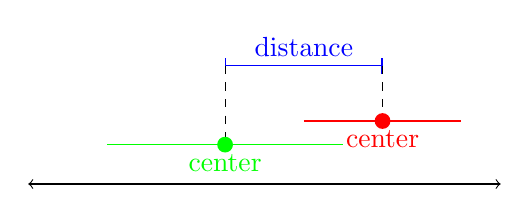
\begin{tikzpicture}
\draw[<->] (0,0) -- (6,0);
\draw[green] (1,0.5) -- (4,0.5);
\draw[red] (3.5,0.8) -- (5.5,0.8);
\draw[|-|, blue] (2.5,1.5) -- (4.5,1.5) node[pos=0.5, above] {distance};
\draw[dashed] (2.5,1.5) -- (2.5,0.5);
\draw[dashed] (4.5,1.5) -- (4.5,0.8);
\fill[green] (2.5,0.5) circle (1mm) node[below] {center};
\fill[red] (4.5,0.8) circle (1mm) node[below] {center};
\end{tikzpicture}
\caption{The distance between Mario's and Koopa's center.}
\end{figure}
\task Since the total of their widths is $1+1.5 = 2.5$, we have the inequality
\[ |x-2.5| < 2.5.\]
\end{tasks}
\end{sol}
\end{frame}


\begin{frame}
\begin{sol}
\begin{tasks}(1)
\task The solutions of
\[ |x-2.5| \leq 2.5\]
are
\begin{eq*}
-2.5 \leq &x-2.5& \leq 2.5 \\
0 \leq &x& \leq 5 \\
&x \in [0,5] &
\end{eq*}
Thus, their hitboxes overlap when $x \in [0,5]$. In other words, they do not overlap when $x \in (-\infty, 0)$ and $x \in (5, \infty)$. Note that this approach results in a cleaner solution than the previous one.
\end{tasks}
\end{sol}
\end{frame}

\begin{frame}
\begin{exercisebox}{}{}
Find the set of solutions for each of the following inequalities.
\begin{enumerate}
\item $|4x-3| <5 $
\item $|x| \geq 2x$
\item $x < |3x-4| < 5x$ (Hint: this implies there are two inequalities. )
\iffalse
\item $|x-1| > |x|$ (Hint: transforming the absolute value one at a time. You should have 4 different inequalities.)
\item (Challenge:) Solve $|x-1| > |x+1|$ using the alternate definition of absolute value function.
\fi
\end{enumerate}
\end{exercisebox}
\end{frame}


%%%%%%%%%%%%%
\section{Quadratic Inequality}
\frame{\sectionpage}
%%%%%%%%%%%%%

\begin{frame}[t]
\frametitle{Observation}
Consider the inequaltiy
\begin{block}{}
\[x^2 - x - 6 > 0\]
\end{block}
We can try plugging in values of $x$ to see what the solutions would look like.
\begin{slide}
\begin{table}
\centering
\begin{tabular}{C||C|C|C|C|C|C|C|C|C}
x & -4 & -3 & -2 & -1 & 0 & 1 & 2 & 3 & 4\\
\hline
x^2-x-6 & 14 & 6 & 0 & -4 & -6 & -6 & -4 & 0 & 6
\end{tabular}
\end{table}
We can guess that the solutions are $x < -2$ and $x > 3$. Likewise, the solution to $x^2-x-6 < 0$ is $-2 < x < 3$. 
\medskip

We will prove that this is the case.
\end{slide}
\end{frame}

\begin{frame}[t]
\frametitle{Motivation}
Suppose we have two real numbers $a$ and $b$ where their product is positive. In other words,
\[ab > 0.\]
\begin{slide}
Then we know that either 
\begin{itemize}
\item They are both positive, or 
\item They are both negative.
\end{itemize}
On the other hand, when the product is negative, or
\[ab < 0,\]
then we know that \textbf{exactly one} of them is positive and the other is negative.
\end{slide}
\end{frame}

\begin{frame}[t]
If we factor $f(x) = a(x-m_1)(x-m_2)$ where $a > 0$, then notice that
\begin{itemize}
\item If $x > m_1$ and $x>m_2$, then both terms are positive. In other words,  
\[x-m_1 > 0 \text{ and } x-m_2 > 0,\]
and thus the product is also positive. Therefore, we have $f(x) > 0$.
\end{itemize}
\begin{figure}[h!]
\centering
\begin{tikzpicture}[scale=0.8]
\draw[<->] (-4,0) -- (4,0);
\node at (-2,-0.5) {$m_1$};
\node at (2,-0.5) {$m_2$};
\draw (-2,0.1) -- (-2,-0.1);
\draw (2,0.1) -- (2,-0.1);
\draw[->, blue, thick] (2,3) -- (4,3);
\draw[->, blue, thick] (2,2) -- (4,2);
\draw[->, blue, thick] (2,1) -- (4,1);
\filldraw[fill = white, draw = blue] (2,3) circle (1mm);
\filldraw[fill = white, draw = blue] (2,2) circle (1mm);
\filldraw[fill = white, draw = blue] (2,1) circle (1mm);
\node at (3,3.2) {$+$};
\node at (3,2.2) {$+$};
\node[above] at (3,1) {$+ \times +$};
\node[below] at (3,1) {$=+$};
\node at (-7,3) {$(x-m_1)$};
\node at (-7,2) {$(x-m_2)$};
\node at (-7,1) {$(x-m_1)\times (x-m_2)$};
\end{tikzpicture}
\caption{A sign of a product when $x > m_2$}
\end{figure}
\end{frame}

\begin{frame}[t]
\begin{itemize}
\item If $m_1 < x < m_2$, then 
\[x-m_1 > 0 \text{ but } x-m_2 < 0.\] 
Hence, the product is negative. Therefore, we have $f(x) < 0$
 \end{itemize}
 \begin{figure}[h!]
\centering
\begin{tikzpicture}[scale=0.8]
\draw[<->] (-4,0) -- (4,0);
\node at (-2,-0.5) {$m_1$};
\node at (2,-0.5) {$m_2$};
\draw (-2,0.1) -- (-2,-0.1);
\draw (2,0.1) -- (2,-0.1);
\draw[blue, thick] (-2,3) -- (2,3);
\draw[red, thick] (-2,2) -- (2,2);
\draw[red, thick] (-2,1) -- (2,1);
\filldraw[fill = white, draw = blue] (2,3) circle (1mm);
\filldraw[fill = white, draw = blue] (-2,3) circle (1mm);
\filldraw[fill = white, draw = red] (2,2) circle (1mm);
\filldraw[fill = white, draw = red] (-2,2) circle (1mm);
\filldraw[fill = white, draw = red] (2,1) circle (1mm);
\filldraw[fill = white, draw = red] (-2,1) circle (1mm);
\node at (0,3.2) {$+$};
\node at (0,2.2) {$-$};
\node[above] at (0,1) {$+ \times -$};
\node[below] at (0,1) {$=-$};
\node at (-7,3) {$(x-m_1)$};
\node at (-7,2) {$(x-m_2)$};
\node at (-7,1) {$(x-m_1)\times (x-m_2)$};
\end{tikzpicture}
\caption{A sign of a product when $m_1 < x < m_2$}
\end{figure}
\end{frame}

\begin{frame}
\begin{itemize}
\item If $x < m_1$ and $x<m_2$, then both terms are negative. In other words,
 \[x-m_1 < 0 \text{ and } x-m_2 < 0,\] 
 and thus the product is still positive. Therefore, we have $f(x) > 0$.
 \end{itemize}
 \begin{figure}[h!]
\centering
\begin{tikzpicture}[scale=0.8]
\draw[<->] (-4,0) -- (4,0);
\node at (-2,-0.5) {$m_1$};
\node at (2,-0.5) {$m_2$};
\draw (-2,0.1) -- (-2,-0.1);
\draw (2,0.1) -- (2,-0.1);
\draw[<-|, red, thick] (-4,3) -- (-2,3);
\draw[<-|, red, thick] (-4,2) -- (-2,2);
\draw[<-|, blue, thick] (-4,1) -- (-2,1);
\filldraw[fill = white, draw = red] (-2,3) circle (1mm);
\filldraw[fill = white, draw = red] (-2,2) circle (1mm);
\filldraw[fill = white, draw = blue] (-2,1) circle (1mm);
\node at (-3,3.2) {$-$};
\node at (-3,2.2) {$-$};
\node[above] at (-3,1) {$-\times -$};
\node[below] at (-3,1) {$=+$};
\node at (-7,3) {$(x-m_1)$};
\node at (-7,2) {$(x-m_2)$};
\node at (-7,1) {$(x-m_1)\times (x-m_2)$};
\end{tikzpicture}
\caption{A sign of a product when $x < m_1$}
\end{figure}
\end{frame}

\begin{frame}
Putting them all together, we have the following complete picture.
\begin{figure}[h!]
\centering
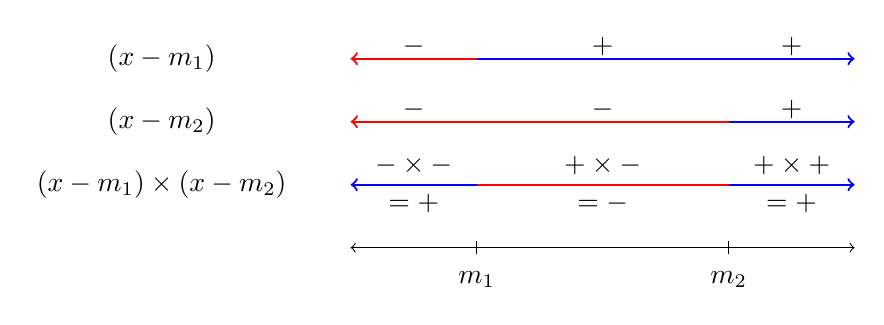
\begin{tikzpicture}[scale=0.8]
\draw[<->] (-4,0) -- (4,0);
\node at (-2,-0.5) {$m_1$};
\node at (2,-0.5) {$m_2$};
\draw (-2,0.1) -- (-2,-0.1);
\draw (2,0.1) -- (2,-0.1);

\draw[->, blue, thick] (-2,3) -- (4,3);
\draw[->, blue, thick] (2,2) -- (4,2);
\draw[->, blue, thick] (2,1) -- (4,1);
\node at (3,3.2) {$+$};
\node at (3,2.2) {$+$};
\node[above] at (3,1) {$+ \times +$};
\node[below] at (3,1) {$=+$};

\draw[<-, red, thick] (-4,3) -- (-2,3);
\draw[<-, red, thick] (-4,2) -- (2,2);
\draw[-, red, thick] (-2,1) -- (2,1);
\node at (0,3.2) {$+$};
\node at (0,2.2) {$-$};
\node[above] at (0,1) {$+ \times -$};
\node[below] at (0,1) {$=-$};

\draw[<-, blue, thick] (-4,1) -- (-2,1);
\node at (-3,3.2) {$-$};
\node at (-3,2.2) {$-$};
\node[above] at (-3,1) {$-\times -$};
\node[below] at (-3,1) {$=+$};

\node at (-7,3) {$(x-m_1)$};
\node at (-7,2) {$(x-m_2)$};
\node at (-7,1) {$(x-m_1)\times (x-m_2)$};
\end{tikzpicture}
\caption{A sign of a product for any real number $x$}
\end{figure}
\end{frame}

\begin{frame}
\frametitle{Solutions of Quadratic Inequality}
\begin{thm}{}{}
Let $f(x) = ax^2 + bx + c$ be a quadratic function. If $a>0$ and 
\[f(x) = a(x-m_1)(x-m_2)\]
where $m_1, m_2$ are the roots of $f(x)$ with $m_1 \leq m_2$, then 
\begin{itemize}
\item The solutions to $f(x) > 0$ are
\[x < m_1 \text{ or } x > m_2.\] 
\item The solutions to $f(x) < 0$ are
\[m_1 < x < m_2.\] 
\end{itemize}
\end{thm}
\end{frame}


\begin{frame}[t]
\begin{ex}
Solve the quadratic inequality
\[x^2 - 3x + 2 < 0.\]
\end{ex}
\begin{sol}
First, we find the roots of the function $f(x) = x^2-3x+2$ and get $x = 1$ and $x=2$. So, we can rewrite the inequality as
\[(x-1)(x-2) < 0\]
\end{sol}
\end{frame}

\begin{frame}
\begin{sol}
\begin{figure}[h!]
\centering
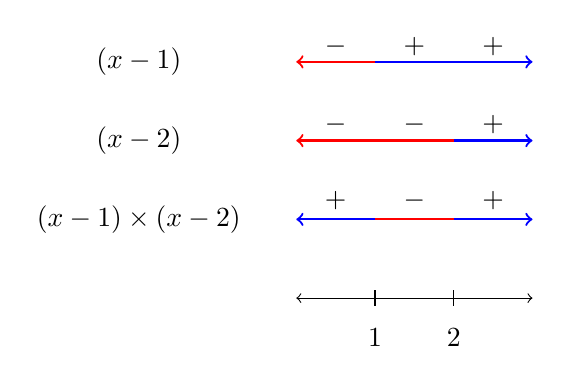
\begin{tikzpicture}
\draw[<->] (0,0) -- (3,0);
\draw (1,0.1) -- (1,-0.1);
\draw (2,0.1) -- (2,-0.1);
\node at (1,-0.5) {1};
\node at (2,-0.5) {2};
\draw[<-, red, thick] (0,3) -- (1,3);
\draw[->, blue, thick] (1,3) -- (3,3);
\draw[<-, red, thick] (0,2) -- (2,2);
\draw[->, blue, thick] (2,2) -- (3,2);
\draw[<-, blue, thick] (0,1) -- (1,1);
\draw[red, thick] (1,1) -- (2,1);
\draw[->, blue, thick] (2,1) -- (3,1);
\node at (0.5,3.2) {$-$};
\node at (1.5,3.2) {$+$};
\node at (2.5,3.2) {$+$};
\node at (0.5,2.2) {$-$};
\node at (1.5,2.2) {$-$};
\node at (2.5,2.2) {$+$};
\node[above] at (0.5,1) {$+$};
\node[above] at (1.5,1) {$-$};
\node[above] at (2.5,1) {$+$};
\node at (-2,3) {$(x-1)$};
\node at (-2,2) {$(x-2)$};
\node at (-2,1) {$(x-1)\times (x-2)$};
\end{tikzpicture}
\caption{The signs of values of $f(x)=x^2-3x+2$ in each interval.}
\end{figure}
Since we want $f(x) < 0$, the solutions are $x \in (1,2)$.
\end{sol}
\end{frame}


\begin{frame}[t]
\begin{ex}
Solve the quadratic inequality
\[x^2 > x.\]
\end{ex}
\begin{sol}
It's tempting to \textit{divide $x$ on both sides}, but please resist it. First, we need to rewrite it as
\[x^2 - x > 0.\]
Then, we can find the roots of the function $f(x) = x^2-x$ to be $x=0$ and $x=1$. Thus, we have
\[x(x-1) > 0.\]
\end{sol}
\end{frame}

\begin{frame}
\begin{sol}
\begin{figure}[h!]
\centering
\begin{tikzpicture}
\draw[<->] (-1,0) -- (2,0);
\draw (1,0.1) -- (1,-0.1);
\draw (0,0.1) -- (0,-0.1);
\node at (0,-0.5) {0};
\node at (1,-0.5) {1};
\draw[<-, red, thick] (-1,3) -- (0,3);
\draw[->, blue, thick] (0,3) -- (2,3);
\draw[<-, red, thick] (-1,2) -- (1,2);
\draw[->, blue, thick] (1,2) -- (2,2);
\draw[<-, blue, thick] (-1,1) -- (0,1);
\draw[red, thick] (0,1) -- (1,1);
\draw[->, blue, thick] (1,1) -- (2,1);
\node at (-0.5,3.2) {$-$};
\node at (0.5,3.2) {$+$};
\node at (1.5,3.2) {$+$};
\node at (-0.5,2.2) {$-$};
\node at (0.5,2.2) {$-$};
\node at (1.5,2.2) {$+$};
\node[above] at (-0.5,1) {$+$};
\node[above] at (0.5,1) {$-$};
\node[above] at (1.5,1) {$+$};
\node at (-3,3) {$x$};
\node at (-3,2) {$(x-1)$};
\node at (-3,1) {$x\times (x-1)$};
\end{tikzpicture}
\caption{The signs of values of $f(x)=x^2-x$ in each interval.}
\end{figure}
Since we want $f(x) > 0$, the solutions are $x<0$ or $x>1$.
\end{sol}
\end{frame}

\begin{frame}
\frametitle{Duplicate roots}
If the roots are the same, then everything we have still holds, with $m_1 = m_2$. For instance
\[(x-m)(x-m) >0\] 
when $x<m$ or $x>m$. In other words, when $x \neq m$.

On the hand,
\[(x-m)(x-m) < 0\]
when $m < x < m$, which implies that there are no solution!
\end{frame}

\begin{frame}
\begin{exercisebox}{}{}
Find the set of solutions for each of the following inequalities.
\begin{enumerate}
\item $x^2 - 9 \geq 0$
\item $x^2+3x+3 < 1$
\item $x^2 > x+2$
\item $2x-x^2 \leq 4-3x$
\end{enumerate}
\end{exercisebox}
\end{frame}

